\chapter{Theorie}
\section{Das Spiel Tic-Tac-Toe}

Tic-Tac-Toe ist ein sehr altes, klassisches Strategiespiel, welches von zwei Personen gespielt wird. Eine Person
spielt hierbei das Symbol Kreuz und eine andere Person das Symbol Kreis. Das Spielfeld von Tic-Tac-Toe besteht aus
neun Feldern, in denen die entsprechenden Symbole verteilt werden können. Jeder Spieler setzt hierzu abwechselnd sein
Symbol in eines der neun Felder. Es ist nicht möglich ein bestehendes Symbol zu überschreiben oder mehrere Symbole in
ein Feld zu zeichnen. Der Anfang einer Runde Tic-Tac-Toe kann beispielsweise wie folgt aussehen:
\begin{figure}[H]
    \centering
    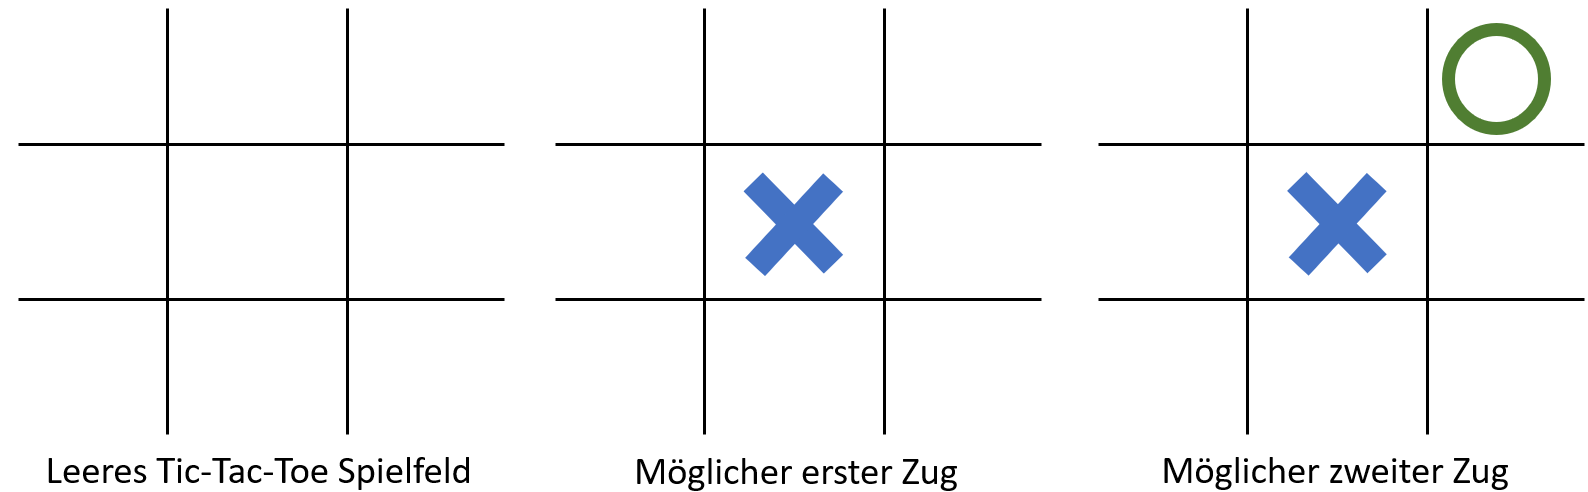
\includegraphics[scale=0.25]{img/tictactoe_start.png}
    \caption[Möglicher Anfang eines Tic-Tac-Toe Spiels]{Möglicher Anfang eines Tic-Tac-Toe Spiels (eigene Anfertigung)}
\end{figure}
Im ersten Teil des Bildes erkennt man die neun leeren Felder des Spielfeldes. Im zweiten Teil des Bildes fängt der erste
Spieler damit an, sein erstes Kreuz in die Mitte des Spielfeldes zu setzen. Der zweite Spieler ist nun am Zug und setzt
im dritten Teil des Bildes seinen Kreis in die obere rechte Ecke des Spielfeldes. Als nächstes wäre Spieler eins wieder an
der Reihe und dürfte sein nächstes Kreuz setzen. Ziel des Spiels ist es, drei gleiche Symbole in einer Reihe, Spalte oder
Diagonale zu haben. Die folgende Abbildung soll dieses Verfahren nochmal genauer erläutern:
\begin{figure}[H]
    \centering
    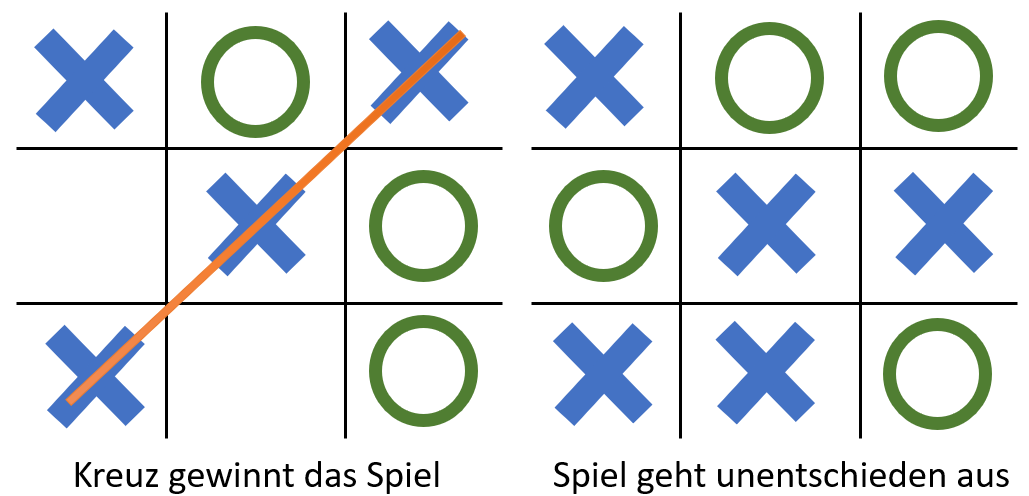
\includegraphics[scale=0.25]{img/tictactoe_endings.png} 
    \caption[Mögliches Ende eines Tic-Tac-Toe Spiels]{Mögliches Ende eines Tic-Tac-Toe Spiels (eigene Anfertigung)}
\end{figure}
Im ersten Teil der Abbildung ist zu sehen, wie der Spieler mit dem Kreuzsymbol drei Kreuze auf einer Diagonale unterbringen
konnte. In diesem Fall ist die Runde beendet und dieser Spieler hat die Runde gewonnen. Ob das Spiel über drei Symbole in einer
Reihe, Spalte oder Diagonale gewonnen wird, ist nicht relevant. Ebenfalls spielt es keine Rolle, in welcher Reihenfolge die 
Symbole gesetzt wurden. Im zweiten Teil des Bildes zeigt sich ein weiteres mögliches Ende für eine Runde Tic-Tac-Toe. Bei diesem
Ende ist das komplette Spielfeld ausgefüllt und es ergeben sich keine drei Symbole in einer Reihe, Spalte oder Diagonale. 
Entsprechend ist die Runde unentschieden ausgegangen.

\section{Der Minimax-Algorithmus}

Der Minimax-Algorithmus, ist ein Algorithmus, der für ein gegebenes Spiel eine Spielstrategie ermittelt. 
Das Spiel muss dabei ein Zwei-Personen-Nullsummenspiel mit perfekter Information sein. Die Idee ist, mögliche 
Spielverläufe zu bewerten und damit für einen gegebenen Spielzustand den Zug zu wählen, der zum besten Spielzustand 
für den zugewiesenen Spieler führt. Als Basis für diese Entscheidung dient eine Funktion utility. Diese Funktion 
nimmt den aktuellen Spielstand und überprüft, in welchem Zustand sich die übergebene Spielsituation befindet. 

\begin{itemize}
    \item Kann im besten Fall ein Sieg erzielt werden, wird der Wert 1 zurückgegeben
    \item Ist nur ein Unentschieden möglich, wird der Wert 0 zurückgegeben
    \item Ist eine Niederlage nicht zu abzuwenden, wird der Wert -1 zurückgegeben
\end{itemize}

Um dies zu ermitteln, wird ein Baum mit allen möglichen Spielverläufen berechnet. Die utility Funktion überprüft 
nun rekursiv für jeden potentiellen Spielzustand, ob das Spiel beendet wurde. Ist dies der Fall, ist das 
Ende des Baumes erreicht und 